\documentclass[11pt, a4paper]{article}
\usepackage{amsmath, color, tikz, xstring}
\usetikzlibrary{calc}

% https://tex.stackexchange.com/questions/49746/a-table-with-square-cells

\def\NumOfColumns{5}%
\def\Sequence{1/A/1/15, 2/B/16/30, 3/C/31/45, 4/D/46/60, 5/E/61/71}%

\newcommand{\Size}{1cm}
\tikzset{Square/.style={
		inner sep=0pt,
		text width=\Size,
		minimum size=\Size,
		draw=black,
		align=center,
	}
}

\begin{document}
	
%	\setlength{\tabcolsep}{18pt} - width of the column
	\setlength{\arrayrulewidth}{1pt} % thick table border
	
	\section{Hello}
	\subsection{Little Text}
	\begin{multline}
		\bigwedge_{\atop i=1}^n \bigwedge_{\atop j=1}^n \bigvee_{\atop k=1}^n
		x_{i,j,k} = (x_{1,1,{\color{red} 1}} \vee \dots \vee x_{1,1,{\color{red} n}}) 
			\wedge (x_{1,2,{\color{red} 1}} \vee \dots \vee x_{1,2,{\color{red} n}})
			\wedge \dots \\
			\wedge (x_{1,n-1,{\color{red} 1}} \vee \dots \vee x_{1,n-1,{\color{red} n}})
			\wedge (x_{1,n,{\color{red} 1}} \vee \dots \vee x_{1,n,{\color{red} n}})
	\end{multline}

	\begin{align*}
		\int_S f \mathrm{d} A &= \sum_{i=1}^n \int_{V_i} f \mathrm{d} A \\
		&- \sum_{i \neq j} \int_{V_i \cap V_j} f \mathrm{d} A \\
		&+ \sum_{i,j,k} \int_{V_i \cap V_j \cap V_k} f \mathrm{d} A\\
		&- \dots
	\end{align*}

	\begin{tabular}{c|c|c|c}
		A & B & C & C \\
		\hline
		A & B & C & C \\
		\hline
		A & B & C & C \\
		\hline
		A & B & C & C \\
	\end{tabular}

	\bigskip


	\let\mc=\multicolumn
	
	\begin{tabular}{c|c|c|c}
		\mc{1}{c}{1} & \mc{1}{c}{2} & \mc{1}{c}{3} & \mc{1}{c}{4} \\ \cline{2-3}
		5 & 2 & 4 & 3 \\ \cline{2-3}
		4 & 3 & 5 & 2 \\ \cline{2-3}
		\mc{1}{c}{1} & \mc{1}{c}{2} & \mc{1}{c}{3} & \mc{1}{c}{4} \\
	\end{tabular}

	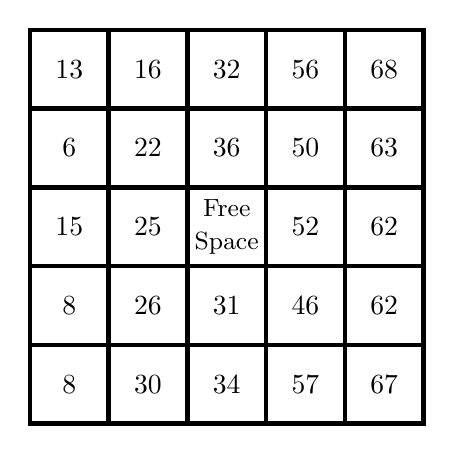
\begin{tikzpicture}[draw=black, ultra thick, x=\Size,y=\Size]
		\foreach \row/\rowLetter/\MinNumber/\MaxNumber in \Sequence{%
			\foreach \col/\colLetter/\MinNumber/\MaxNumber in \Sequence {%
				\pgfmathtruncatemacro{\value}{\col+\NumOfColumns*(\row-1)}
				\def\NodeText{\pgfmathparse{random(\MinNumber,\MaxNumber)}\pgfmathresult}
				\pgfmathsetmacro{\ColRowProduce}{\col*\row}
				\IfEq{\ColRowProduce}{9}{% If is center square
					\node [Square] at ($(\col,-\row)-(0.5,0.5)$) {\small Free Space};
				}{
					\node [Square] at ($(\col,-\row)-(0.5,0.5)$) {\text \NodeText};
				}
			}
		}
	\end{tikzpicture}


\end{document}